\section{Genomförande}
Modellprovaren skrevs i prolog då det är ett lämpligt programmeringsspråk för bevissökning. De befintliga reglerna för CTL implementerades. Vissa av reglerna kräver variabelt antal premisser och detta måste hanteras av programmet. Implementationen av reglerna och modellprovaren gås igenom i kapitel~\ref{sub:modellprovaren}. I kapitel~\ref{sub:modell} beskrivs vår egenvalda modell som föreställer ett trafikljus.

\begin{figure}[hb]
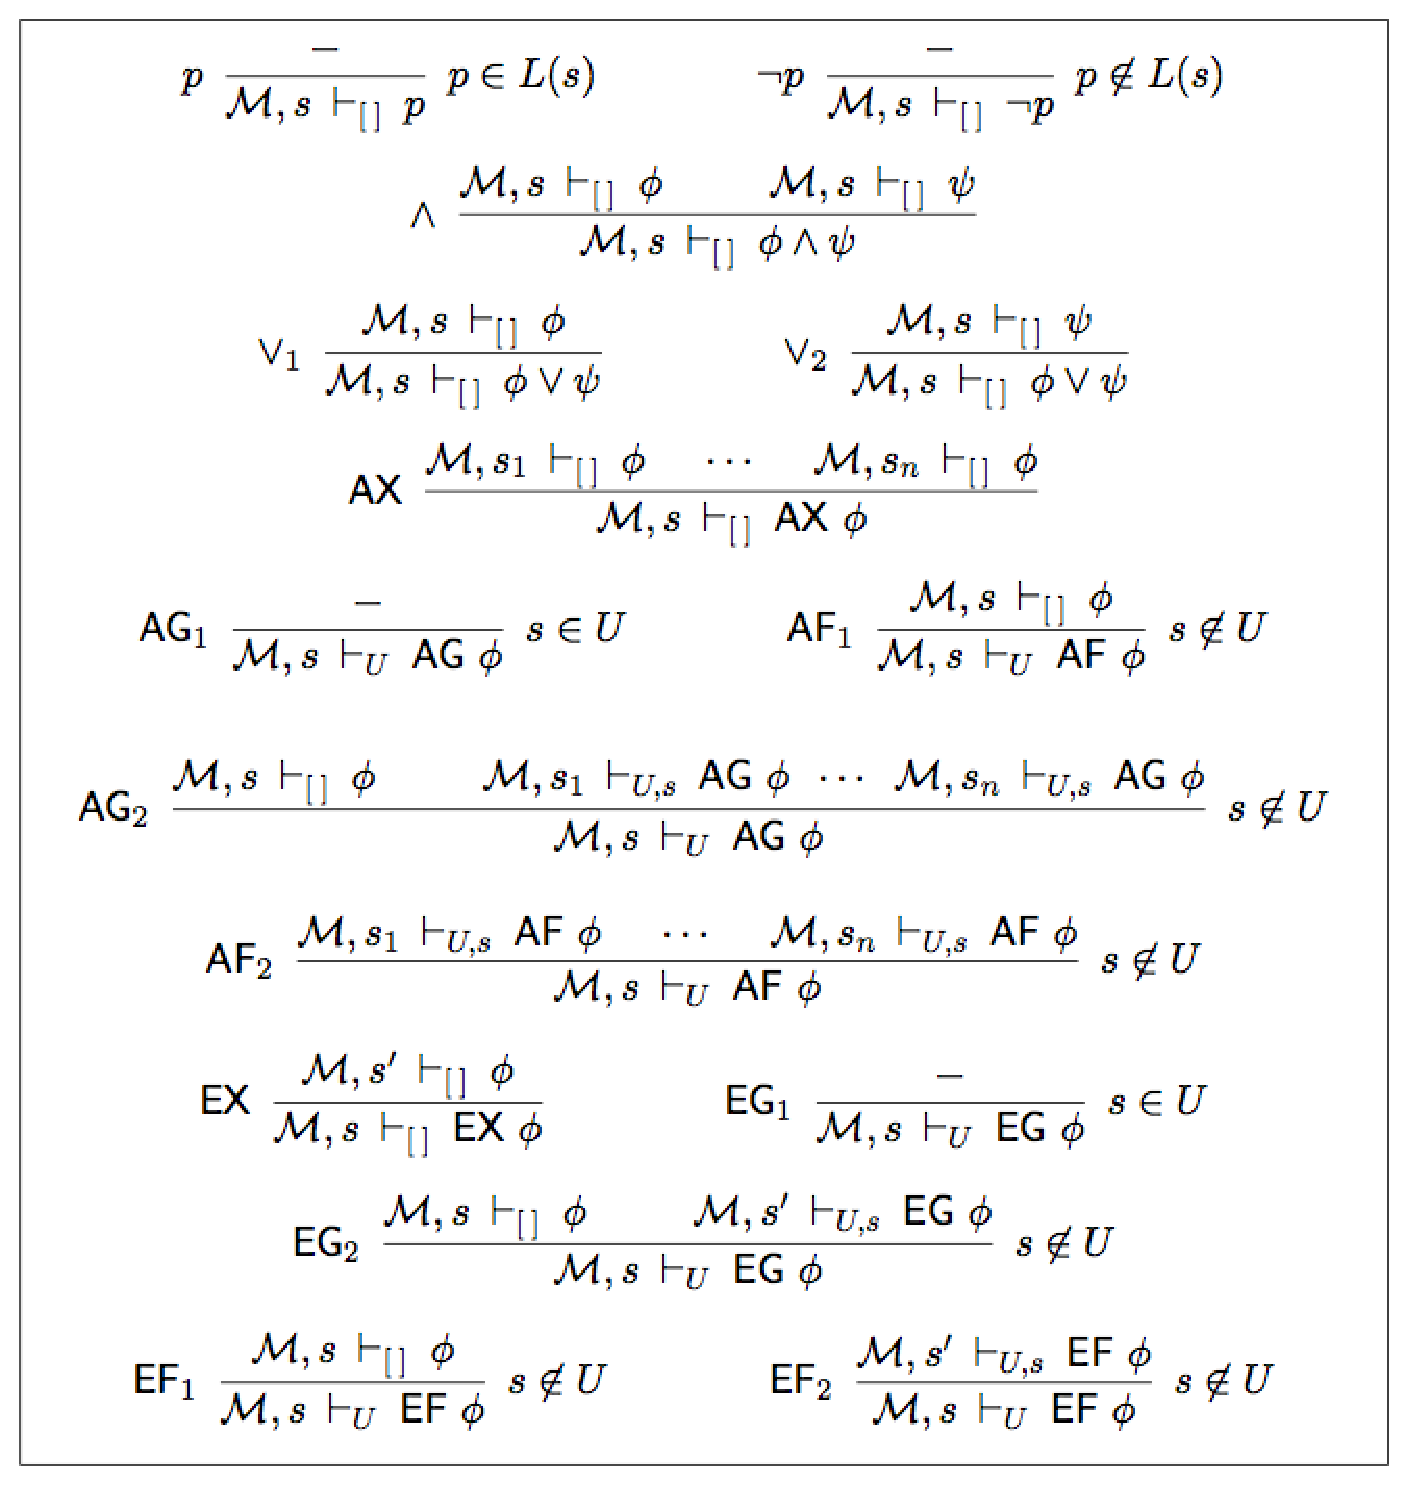
\includegraphics[width=\textwidth]{formulas.eps}
\caption{Regler för CTL}
\label{fig:ctl-regler}
\end{figure}
\subsection{Modellprovaren}\label{sub:modellprovaren}

För att kunna testa modellprovaren fanns flertalet tester att tillgå som bestod av en liststruktur för att beskriva tillståndens egenskaper och grannar, detta beskrivs tydligare under Modell.
Programmet skrevs så att en funktion “check” anropades med följande inparametrar:

\begin{center}
\begin{minipage}{0.75\textwidth}
\texttt{check(T, L, S, U, F)}

\texttt{T - Alla tillstånd och dess grannar i listform}

\texttt{L - Lista över egenskaper i varje tillstånd}

\texttt{S - Aktuellt tillstånd}

\texttt{U - Lista för besökta tillstånd}

\texttt{F - CTL formel som ska testas}

\end{minipage}
\end{center}

Check skrevs så att den med pattern matching kan matchas mot alla de regler som skulle implementeras. De matchades på följande sätt: \texttt{X}, \texttt{neg(X)}, \texttt{and(F,G)}, \texttt{or(F,G)}, \texttt{ax(X)}, \texttt{ag(X)}, \texttt{ex(X)}, \texttt{eg(X)}, \texttt{ef(X)}.

Nedan följer ett utrag ur programkoden för kontroll av \texttt{ef(X)}:

\begin{center}
\begin{minipage}{0.6\textwidth}

\begin{lstlisting}
% EF 1
check(T, L, S, U, ef(X)) :-
	not(member(S, U)),
	check(T, L, S, [], X).

% EF 2
check(T, L, S, U, ef(X)) :-
	not(member(S, U)),
	member([S, Srest], T),
	echeck(T, L, Srest, [S|U], ef(X)).
\end{lstlisting}


\end{minipage}
\end{center}


Då check stötte på \texttt{ef(X)} försökte den först med implementationen EF1 och
sedan om den evaluerades till false försökte den med EF2.

EF1 skrevs så att den alltid kontrollerar att nuvarande tillstånd \textit{S} inte finns bland tidigare besökta \textit{U} och fortsätter sedan rekursivt med resten av beviset \textit{X} och tömd lista \textit{U} för tidigare besökta tillstånd. Detta uppfyller kraven för regel EF1 som kan ses i figur 1.

EF2 skrevs så att den på samma sätt som EF1 kontrollerar att \textit{S} inte
tidigare har besökts. I nästa steg kontrollerar den vilka grannar \textit{S} har
övergångar till och skickar med dessa till funktionen echeck. Denna funktion kontrollerar att
någon av tillståndets \textit{S} grannar evalueras till sant. Till echeck skickas även en lista innehållandes tidigare besökta tillstånd där nuvarande tillståndet \textit{S} läggs till. Detta uppfyller
kraven för EF2.

De resterande reglerna från figur~\ref{fig:ctl-regler} implementerades på liknande sätt och dessa kan ses i den bifogade koden under kapitel~\ref{bilagor}.

\subsection{Modell}\label{sub:modell}

